\chapter{\textsc{Modélisation du système Segment Piston Chemise (SPC)}}\label{Modelisation}
La compréhension du comportement des surfaces en contact dans les système \emph{SPC}, a une importance capitale dans l'amélioration de performance du moteur à combustion interne comme nous le verrons plus loin dans l'exposé. La lubrification qui se produit dans l'interface \emph{SPC} impose une certaine forme assez particulière de mode de lubrification qui couvre le régime mixte, hydrodynamique et critique (Chapitre \ref{generalite}). Ainsi pour la tribologie. On peut classer les défauts en fonction de leur longueurs d’onde $L$ Image \ref{fig:ondulation}  \cite{initiation} :

\section{Caractérisation de la topographie de la chemise}
La prise en compte de la caractérisation de la surface, influence en grande partie sur les performances du moteur. celle-ci influence la qualité de la séparation du contact mais aussi le transport du lubrifiant par les segments le long de la chemise.\\

Il existe plusieurs théories qui expliquent les phénomènes de frottement dans la littérature. Parmi celles-ci, trois approches majeures se distinguent : la théorie de la \textbf{rugosité}, qui s'intéresse aux irrégularités de surface ; la théorie de l'\textbf{attraction moléculaire}, qui met en évidence les forces d'attraction entre les molécules des surfaces en contact ; et enfin, la théorie de \textbf{l'adhésion}, qui se concentre sur les interactions directes au niveau microscopique entre les matériaux. Parmi ces théories, celle de l'adhésion de Tabor et Bowden est souvent considérée comme la plus précise, car elle prend en compte une gamme complète de paramètres influençant les frottements. Cependant, nous avons choisi d'adopter la théorie de la \textbf{rugosité} pour cette étude, car elle est plus simple à intégrer dans notre modèle, tout en étant suffisamment représentative pour les applications liées aux moteurs à combustion interne (MCI). De plus, la théorie de l'adhésion de Tabor et Bowden est surtout appliquée dans le domaine des matériaux composites et des surfaces, plutôt que directement dans les moteurs à combustion interne.\\

Dans la suite, gardons à l'esprit que la prise en compte des effets de la rugosité en lubrification des corps en mouvement relatif, est un problème assez compliqué faisant intervenir de nombreux aspect ; entre autre le caractère changeant du domaine occupé par le fluide en mouvement relatif, ou la déformation de surface de corps en mouvement relatif. En outre les difficultés liées à la physique des fluides, qui peut être plus ou moins complexe suivant les cas ou la nature du lubrifiant : effets de compressibilité, effets piézovisqueux, cavitation, couplage avec la thermique pour ne cité que çà. Aussi, une autre difficulté est liée à la différence nette entre l'échelle de grandeur de la rugosité et celle de l'ingénieur qui est généralement de plusieurs ordres de grandeur plus grandes que celle de la rugosité (généralement inférieur à $0.001\%$ )\cite{initiation}.\\

Quelque soit le moyen de mise en oeuvre utilisé, les surfaces présentent des écarts géométriques par rapport à leur forme théorique.Ces défauts jouent un rôle primordial en tribologie. On peut classer les défauts en fonction de leur longueurs d'onde la (Figure \ref{fig:ondulation})
\begin{itemize}
	\item si $L$ est de l’ordre de la taille de la surface, on parle de défaut de forme ;
	\item Lorsque $0.001m < L < 0.01m$, on parle de defaut d'ondulation;
	\item les défauts de longueur d’onde inférieur sont appelés rugosité.
\end{itemize}
% TODO: \usepackage{graphicx} required
\begin{figure}
	\centering
	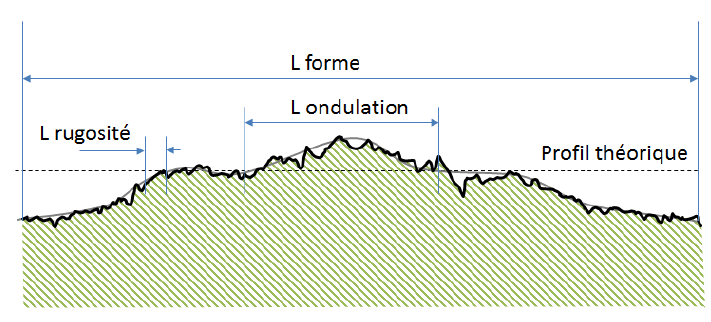
\includegraphics[width=0.7\linewidth]{Img/ondulation}
	\caption[Défaut géométrique du surfacee]{Défaut géométrique du surface}
	\label{fig:ondulation}
\end{figure}
La rugosité est donc l'ensemble des irrégularités microscopique et macroscopique d'une surface.
Toutes les surfaces, naturel ou fabriqué, ne sont pas parfaitement lisses. La surface la plus
douce dans les corps normaux est celle du \emph{mica}. Le \emph{mica} a une rugosité approximativement de $0.002032 microns$.\cite{ayad1}

\subsection{Méthodes des texturations des chemises}
\lettrine{L}{a} majeur partie des pièces de moteur vient de l'industrie métallurgique. Dans leur procéder de fabrication plusieurs méthodes de finissage de la surface sont employées. Le principale étant l'abrasion par \emph{galetage} \footnote{Techniquqe de finissage  de la surface qui peut avoir plusieurs objectifs comme le renforcement mécanique de la surface} et \emph{ grenaillage} \footnote{c'est une technique qui consiste à projeter à grande vitesse des billes sur la surface d'un objet pour en modifier la structure superficielle, a fin d'améliorer l'aspect et les caractéristiques techniques.} sont les premières opérations qui vont permettre une maîtrise de rugosité jusqu’à un ordre de grandeur de 0.5mm.\cite{ayad1} À partir de l’état de surface obtenu, on cherchera à introduire une "texturation" qui va permettre de créer une rugosité plus "précise" sur l’interface de la surface (figure \ref{fig:caracterisation}).
% TODO: \usepackage{graphicx} required
\begin{figure}[h]
	\centering
	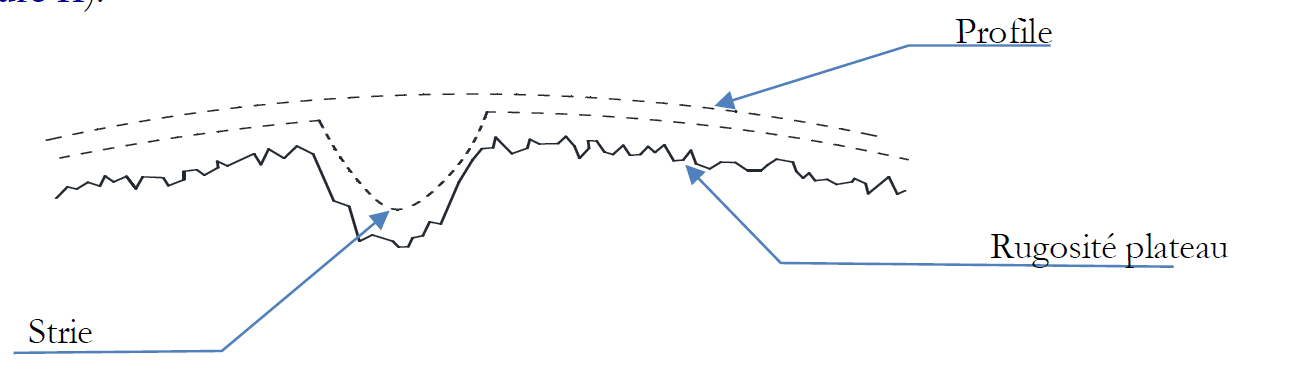
\includegraphics[width=0.7\linewidth]{Img/caracterisation}
	\caption[surface texturée]{Profil de rugosité de surface texturée}
	\label{fig:caracterisation}
\end{figure}
\subsubsection{Texturation avec procédé chimique}
\lettrine{D}{ans} cette technique, un film protecteur est posé sur la surface de la pièce. Ce film est muni de motif par lequel un acide va s’infiltrer pour attaquer l’interface. La concentration utilisée et le temps laissé avant le rinçage déterminent la profondeur de la texture souhaitée. Cette technique a l’avantage de ne pas entraîner de déformation du matériau autour de la texture, de ne pas générer de débris pouvant subsister dans le contact, mais elle est très lourde à mettre en place sur une chaîne de production, car il faut isoler toutes les parties qui ne seront pas concernés par la texturation.
\subsubsection{Texturation à l'aide d'un diamant}
\lettrine{D}{ans} ce procédé d’usinage, un diamant est utilisé pour réaliser la texturation, 3 paramètres permettent de contrôler la texture obtenue :
\begin{itemize}	
	\item La vitesse de deplacement verticale;
	\item La vitesse de rotation du rodoir;
	\item La vitesse d'abrasion des diamants.
\end{itemize}
Ce procédé a plusieurs avantages : rapidité, bonne finition, peu coûteux, facile à mettre en place sur les chaînes de production, mais la surface s’en trouve légèrement déformée autour de la texture.

\subsection{Paramètres de rugosités}
\lettrine{L}{e} Tout premier appareil de mesure du profil de la surface est le palpeur en diamant. Cette appareil se déplace longitudinalement sur la face en donnant généralement un ensemble des points $n$ de variation de la hauteur $z_i$ espacé d'une intervalle latéral $\delta x$. A partir de cette série, on peut calculer des paramètres d’amplitude. Le plus utilisé dans la communauté des mécaniciens est le $R_a$ \cite{initiation}. Pendans longtemps un seul paramètre était connu et utilisé $R_a$ (Routhness Average), d'autres paramètres sont venus après comme RMS(Rout Mean Squart). Aujourd'hui, les paramètres de mesure de surface sont définis suivant plusieurs normes internationales où il y a même des variantes sectorielles (la sidérurgie ou l'automobile). On distingue trois groupes de paramètres de mesure utilisés selon le type de profil \cite{ayad1}:
\begin{itemize}
	\item Paramètres de préfixe P calculés sur le \textbf{profil primaire};
	\item Paramètres de préfixe R calculés sur le \textbf{profil de rugosité} ;
	\item Paramètres de préfixe W calculés sur le \textbf{profil d'ondulation}.
\end{itemize}
Dans le cadre notre travail; nous allons être indulgent envers nous-même en limitant notre travail dans l'étude de la surface  par le préfixe de R du \emph{profil de rugosité} pour simplifier le travail.\\

La figure \ref{fig:profil-surface} présente un exemple de profil de surface. L’échelle verticale est amplifiée par rapport à l’échelle horizontale pour que les rugosités puissent être discernées. En coupant le profil par une ligne horizontale, il est possible de calculer le pourcentage de points situés au dessus de la ligne. En balayant verticalement le profil avec la ligne horizontale, on obtient l’évolution de ce pourcentage en fonction de la hauteur $z$. La courbe obtenu est appelée \emph{courbe de portance} ou \emph{courbe d'Abbott} (Figure \ref{fig:analysedistribution}). Elle indique le pourcentage de points qui entrerait en contact avec un plan rigide situé à la hauteur $z$.\cite{initiation}
% TODO: \usepackage{graphicx} required
\begin{figure}[h]
	\centering
	\includegraphics[width=0.7\linewidth]{"Img/profil surface"}
	\caption[profil surface]{Profil de surface}
	\label{fig:profil-surface}
\end{figure}
% TODO: \usepackage{graphicx} required
\begin{figure}[h]
	\centering
	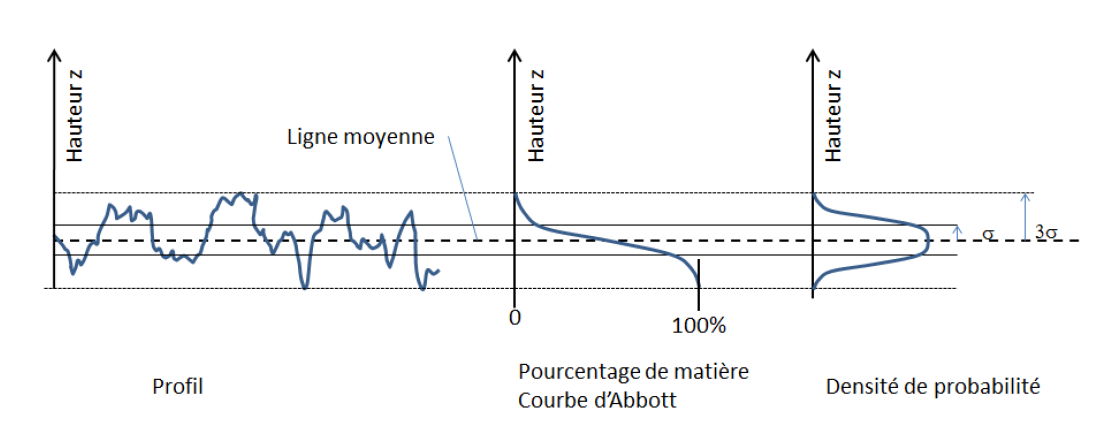
\includegraphics[width=0.7\linewidth]{Img/analysedistribution}
	\caption[analyseRigosité]{Analyse de rigosité}
	\label{fig:analysedistribution}
\end{figure}

Les paramètres d’évaluation de la topographie d’une surface sont référencés par une lettre majuscule R indicé d’une lettre minuscule propre au paramètre. Dans le soucis de la préservation de la tradition du métier de mécanicien, nous allons garder la même notation :
\begin{equation}
	{R}_{a}=\frac{1}{n}\sum _{1}^{n}\left|z_i\right|
	\label{Ra}
\end{equation}
\begin{equation}
	{R}_{a}=\frac{1}{L}{\int }_{0}^{L}\left|z\right|dx
\end{equation}
On utilise également $R_q$ ou RMS:
\begin{equation}
		{R}_{q}=\sqrt{\frac{1}{n}\sum _{1}^{a}{z_i}^{2}}
\end{equation}
\begin{equation}
		{R}_{q}=\sqrt{\frac{1}{L}{\int }_{0}^{L}{z}^{2}}
\end{equation}

Ce paramètre $R_q$ est équivalent à l’écart type, on utilisons aussi un paramètre de symétrie
\begin{equation}
	RSk=\frac{1}{n{R}_{q}^{3}}\sum {z}_{i}^{3}
\end{equation}
\begin{equation}
	RSk=\frac{1}{L{R}_{q}^{3}}\underset{0}{\int }{z}^{3}\left(x\right)dx
\end{equation}
Une valeur positive de ce paramètre indique des pics plus marqués que les vallées. La
situation inverse correspond à une valeur négative de $RSk$. Enfin, le paramètre d’étalement
indique sur quelle étendue sont distribués les points de la surface. Koshy et Tovey (2011) ont montré que l'asymétrie et la kurtosis (applatissement) sont de bons indicateurs de la réduction de la friction sur la face de coupe des outils, particulièrement après une modification de la rugosité via l'usinage par décharge électrique\cite{trobo2} :
\begin{equation}
	RKu=\frac{1}{n{R_q}^{4}}\Sigma {z}_{i}^{4}
\end{equation}
\begin{equation}
	RKu=\frac{1}{L{R_q}^{4}}\int_{0}^{L}{z}_{i}^{4}
\end{equation}
\section{Modélisation de la surface de la chemise}
La surface d’une chemise texturée, est composée d’une micro géométrie comportant des stries de géométrie bien définie, reparties de façon régulière sur des plateaux rugueux qui les séparent (Figure \ref{fig:image-topographique}. Une chemise non-texturée comporte uniquement la rugosité des plateaux.\\

Les stries forment des motifs uniformes qui se répètent de manière alternative sur toute la surface de la chemise. Dans le souci de calcule, il sera très difficile de discretiser toute la chemise car elle vas nécessiter un grand nombre de calcule pour l'ordinateur. En effet, pour une largeur de strie de $100 \mu m$ prise sur une hauteur de $10 cm$ et un périmètre de $25 cm$, il faudrait utiliser une grille de 50 000 x 20 000 points pour représenter correctement chaque strie (~ 20 points par strie), ce qui entraînent un temps de calcul machine de plusieurs jours voire des semaines. Mais comme les motifs de texturation se répètent de manière cyclique, la chemise peut être assimilée à un plan infini dans le sens circonférence, ce qui donne la possibilité de prendre un motif élémentaire de la texturation complète.\\

En ce qui concerne les rugosités des plateaux et des segments, l’ordre de grandeur de la hauteur moyenne des aspérités\footnote{Rugosités de plateau} est inférieur à la profondeur des stries de texturation, l’influence de leurs rugosités sur la lubrification peut donc être étudiée séparément en utilisant un modèle statistique, qui détermine la pressions moyenne du contact des aspérités entre les surfaces


\section{Rôle de la topographie de la chemise}
La topographie de la surface du cylindre joue un rôle essentiel dans le cadre du contact
segments-piston-chemise et influence considérablement la lubrification et le frottement ;
elle est souvent le résultat d’un compromis entre une bonne isolation de la chambre de
combustion et une bonne lubrification du cylindre.\\

La texture des surfaces affects la pression généré dans le contact segment chemise ainsi que
l'huile qui coule à travers. En expliquant l'effet des aspérités sur le frottement de la segmentation, on peut donc contrôler ses effets indésirables, pour cela on a supposé que la distribution de la rugosité sur la chemise et le segment est isotropique et gaussienne en nature.\\

Dans le monde aujourd'hui, il existe un consensus dans le monde automobile concernant la texture des chemises des cylindres ; la texture classique est constituée de plateaux lisses et réguliers,
séparés par des stries de lubrification. Les images de la (Figure \ref{fig:image-topographique}) montrent un exemple de surface de cylindre et ont été acquises par relevé topographique à l’aide d’un palpeur mécanique.\cite{costin}.

\begin{figure}[h]
	\centering
	\includegraphics[width=0.7\linewidth]{"Img/image topographique"}
	\caption[exemple de texture de surface]{exemple de texture de surface}
	\label{fig:image-topographique}
\end{figure}

pour obtenir ce genre de surface, la pièce doit être usinée généralement de la manière suivante :
\begin{enumerate}
	\item alésage, pour donner la géométrie du cylindre ;
	\item pour donner la géométrie du cylindre ;
	\item rodage fin, pour obtenir la rugosité désirée ;
	\item rodage de plateaux, pour le lissage.
\end{enumerate}

\section{Lubrification dans le Segment et le piston }
Tout au long de notre travail nous avons décrit le comportement du systeme SPC. durant cette section nous allons modeliser le comportement de l'huile en prenant en compte les exigences du comportement de fonctionnement du syteme.\\

Tout au long du cycle du moteur, chaque segment est soumis à un mode de lubrification différent en raison de la variation d’approvisionnement en huile. Ces modes de la lubrification ont un important effet sur la force de frottement produite par le mouvement des segments le long de la chemise. \\

Tels que vue dans la (section \ref{spc}) La lubrification sera dite limite lorsque les deux surfaces sont en contactent directement, sinon bien evidamment les deux surfaces seront séparées par une quantité d'huile suffisant soutenant la charge due au segment dans ce cas nous parlerons de la lubrification hydrodynamique.Il existe une zone entre les deux où la charge est supportée par le lubrifiant et les aspérités, dans ce cas-là on parle de régime mixte. \\

Les modes de lubrification sont caractérisés par un espacement entre les lignes nominales des deux surfaces du triplet. Selon la distance entre les lignes nominales h(x) la (figure \ref{fig:mode-delubrification-par-le-triplet}), trois modes de lubrification sont possible :\\
\begin{itemize}
	\item Lubrification Hydrodynamique si $H_{\sigma} > 3 $;
	\item Lubrification limite si $H_{\sigma}<1$;
	\item Lubrification mixe $1<H_{\sigma} < 3$.
\end{itemize}
avec : $$ H_{\sigma} = \frac{h_{T}}{\sigma} $$
Et 
\begin{equation}
	\sigma =\sqrt{{R}_{q}_{segment}^{2}+{R}_{q}_{chemise}^{2}}
\end{equation}

% TODO: \usepackage{graphicx} required
\begin{figure}[h]
	\centering
	\includegraphics[width=0.7\linewidth]{"Img/mode delubrification par le triplet"}
	\caption[Etat de lubrification triplet]{}
	\label{fig:mode-delubrification-par-le-triplet}
\end{figure}

\subsection{Equation de Reynold}
L’équations qui régi le comportement du film d'huile entre segment et chemise est l’équation de base de la lubrification hydrodynamique dite équation de Reynolds\cite{tribo1}. Cette équation relie la taille, la largeur et la forme du film d'huile entre le segment et la chemise, avec le gradient de pression qui se produit dedans et est données dans sa forme la plus générale par :

\begin{equation}
	\frac{\partial }{\partial x}(\rho \frac{h^3}{\mu}\frac{\partial p}{\partial x})+ \frac{\partial}{\partial y}(\frac{\rho h^3}{\mu}\frac{\partial p}{\partial y})=6\frac{\partial}{\partial x}[(U_{1}+U_{2})\rho h] +6\frac{\partial}{\partial x}[(V_{1}+V_{2})\rho h]+ 12 \frac{\partial}{\partial t}(\rho h)
	\label{equation-generale-raynold}
\end{equation}
Dans cette équation nous exprimons bien évidement la variation de h en fonction de temps comme :
\begin{equation}
	\frac{\partial h}{\partial t} =W_{1}-U_{2}\frac{\partial h_{2}}{\partial x}- V_{2}\frac{\partial h_{2}}{\partial y}- W_{1}+U_{1}\frac{\partial h_{1}}{\partial x}+V_{1}\frac{\partial h_{1}}{\partial y}
\end{equation}

Notons que l’équation présentée ici est valable pour des fluides compressibles ou incompressibles dont
la viscosité ne varie pas suivant z en outre il decoule de l'équation de Navier-Stokes. Il est utile de rappeler les hypothèses ayant permis d’établir cette équation :
\begin{itemize}
	\item Le fluide est Newtonien de viscosité constante suivant h ;
	\item La densité du fluide est constante suivant h ;
	\item Le fluide adhère parfaitement aux parois ;
	\item L’écoulement est laminaire et le nombre de Reynolds suffisamment petit pour que
	l’inertie du fluide soit négligeable ;
	\item Le milieu est continu.
\end{itemize}
Dans le cadre de notre travail, une étude en 2-D est employée, dans laquelle les paramètres définissant la lubrification du contact sont déterminés sur des endroits circonférentiels spécifiques du piston et l'équation de Reynolds se réduit ainsi à une forme 1-D à chacun de ces endroits, et en plaçant l'origine du système d'axe sur l'une des parois du contact, l'équation (\ref{equation-generale-raynold}) devient donc :
\begin{equation}
	\frac{\partial}{\partial x}{(\frac{h^3}{\mu}\frac{dp}{dx})}=6U\frac{\partial h}{\partial x}+12\frac{\partial h}{\partial t}
	\label{eq-reduite-raynold}
\end{equation}
$p$ étant la pression hydrodynamique dans le film d'huile, $\mu$ la viscosité dynamique de l'huile, $h$ épaisseur du film d'huile sous les segments, $U$ la vitesse de rotation. ainsi nous obtenons une équation beaucoup plus potable.

\subsection{Equation de Reynold Modifiée}
Le modèle de lubrification dynamique proposé par Patir et Cheng repose sur une adaptation de la théorie classique de Greenwood et Williamson, qui décrit les contacts entre surfaces rugueuses. Leur approche modifie les équations classiques pour inclure les effets de rugosité en utilisant des facteurs correctifs pour le débit et la pression à travers les micro-cavités des surfaces en contact. Cette méthode permet d'intégrer à la fois les effets hydrodynamiques et ceux dus à la micro-géométrie des aspérités, rendant le modèle plus réaliste pour des applications pratiques, notamment dans des conditions de lubrification mixte.\cite{tribo1}
\begin{equation}
	\frac{\partial}{\partial x}(\phi_{x} \frac{h^3}{\mu_{m}} \frac{\partial p}{\partial x}) = \frac{U}{2} \frac{\partial}{\partial x}(h_{T}-\partial \phi_{s})+\frac{\partial h_{T}}{\partial t}
	\label{eq_reynold_modifie}
\end{equation}
si Nous prenons 
$$ U \frac{\partial h}{\partial x} \sim LN \frac{h}{b}$$
Et aussi 
$$\frac{\partial h}{\partial t} \sim hN $$
en faisant le rapport de ce deux nous obtenons donc 
$$ \frac{\frac{\partial h}{\partial t}}{U\frac{\partial h}{\partial x}} \sim \frac{b}{L}<< 1 $$
Cette maneuvre viser à reduire l'équation de Reynold tels que modifiée, cette simplification est vqlide dans toute les parties du cycle, ainsi l'équation (\ref{eq_reynold_modifie}) devient donc :
\begin{equation}
	\frac{\partial}{\partial x}\left(\phi_{x} \frac{h^3}{\mu_{m}} \frac{dp}{dx}\right) =\frac{U}{2}\left(h_{T}-\sigma \phi_{s}\right)
	\label{eq_reynold_simplifie}
\end{equation}
\begin{itemize}
	\item $N$ est la vitesse du moteur en tr/s ;
	\item $L$ est la longueur de la course ;
	\item $h$ est l'épaisseur de film d'huile sous le segment ;
	\item $U$ est la vitesse de piston ;
	\item $\mu_{m}$ est la viscosité dynamique du lubrifiant ;
	\item $b$ est la taille axiale du segment.
\end{itemize}
La vitesse instantanée U du piston peut être décrite par une fonction quasi harmonique de la position angulaire θ du vilebrequin, en relation avec la vitesse angulaire ω, conformément à l'expression :
\begin{equation}
	U =\frac{R}{b}\sin{\theta} \left(1-\frac{\cos\theta}{\sqrt{(\frac{L}{b})^2-\sin\theta}}\right)b\omega
\end{equation}
La vitesse angulaire est elle‐même liée à la vitesse du moteur par la relation :
\begin{equation}
	\omega =\frac{2\pi}{60}N
\end{equation}
